\chapter{INTRODUCTION}

% \pagestyle{plain}

\label{ch:intro}

TODO

%%%%%%%%%%%%%%%%%%%%%%%%%%%%%%%%%%%%%%%%%%%%%%%%%%%%%%%%
\section{Electrical Source Imaging Framework}

TODO: Better intro to the intro

cite the review from Hllez\cite{hallez2007review}.

    

%%%%%%%%%%%%%%%%%%%%%%%%%%%%%%%%%%%%%%%%%%%%%%%%%%%%%%%%
%%%%%%%%%%%%%%%%%%%%%%%%%%%%%%%%%%%%%%%%%%%%%%%%%%%%%%%%

\section{Derivation of the forward model}

Electroencephalography (EEG) consists of the collocation of surface electrodes, whose surface is in the order of 20 \si{mm^2}, on the subjects' exposed scalp.
%
The recording circuit is often completed by setting a reference electrode at either a 'neutral' location or another electrode; the discussion of an appropriate reference electrode location can be skipped by re-referencing the recordings against their average.

Within the distributed dipole paradigm, we assume that the electric scalar potential field is caused exclusively by a finite collection of electric dipoles. 
%
Such an assumption derives from the fact that post-synaptic potentials on neurons can be approximated as electric dipoles at a reasonable distance.

It is reasonable to state that the electric scalar field obtained by the EEG is caused by the numerous electrical dipoles created by neurons' post-synaptic potentials.
%
However, we must consider that those dipoles are small and far away from the sensors --to the size of EEG sensors.
%
This is in addition to the attenuation due to the tissues between the neurons and the EEG sensors and the possibility of silent sources whose total summation is close to zero due to their relative orientation.
%
As the transition from neuron dipoles to EEG sensors loses information, activity from low-entropy regions can be recovered under appropriate assumptions.

%%%%%%%%%%%%%%%%%%%%%%%%%%%%%%%%%%%%%%%%%%%%%%%%%%%%%%%%
%%%%%%%%%%%%%%%%%%%%%%%%%%%%%%%%%%%%%%%%%%%%%%%%%%%%%%%%

\subsection{Derivation of the Poisson equation}

EEG sensors register the electric scalar potential field, $V: \R^3 \rightarrow \R$, at numerous points in space, $s_{1}, s_2, \dots, s_M \in \R^3$; i.e., $V(s_m)$ represents the measurement from the $m$-th sensor.
%
As it is discussed in the previous section, we assume that the electric scalar potential field is caused by a finite number of dipoles with known locations ($d_1, d_2, \dots, d_N \in \R^3$) and whose momentum ($m_1, m_2, \dots m_N$) are to be determined.

We first consider a single dipole with unit magnitude and a single sensor to model the interactions between the dipoles and the sensors. The whole model is later constructed by superposition.

Under these circumstances, we consider the electric field, $E: \R^3 \rightarrow \R^3$, and the current density field, $K: \R^3 \rightarrow \R^3$,
\begin{align}
E &= - \nabla V
\\
K &= \sigma E = - \sigma \nabla V
\label{eq:model1}
\end{align}
with $\sigma: \R^3 \rightarrow \R^{3\times 3}$ the position-dependent conductivity tensor. 
%
In the isotropic case, we assume
$\sigma(r) = \kappa Id$
for all $r$ and some constant conductivity $\kappa>0$.

The current density field has the property that its divergence vanishes everywhere except near the dipole.
%
In more precise terms, the divergence of the current density field is defined as
\begin{equation}
\nabla \cdot K = \lim_{G(r) \rightarrow \sset{r}} \frac{1}{\text{vol}\ppar{G\ppar{r}}}
\oint_{\partial G(r)} K(r)\, dS
\end{equation}
whit $G(r)\subset \R^3$ a set that contains $r$; the limit must be interpreted in a similar way as Riemann sums, in the sense that the limit is not affected by the selections of $G(r)$ when it does exist.
%
For the case of one single dipole, $\nabla \cdot K$ can be simplified,
\begin{equation}
\nabla \cdot K(\rr) = {\delta\ppar{r-\rr_+} - \delta\ppar{r-\rr_-}} =
\begin{cases}
+1, &\text{if } r=r_+ \\
-1, &\text{if } r=r_- \\
0, &\text{otherwise}.
\end{cases}
\label{eq:model2}
\end{equation}
with $r_-, r_+ \in \R^3$ the electric sink and source positions, respectively, related to the single source. 
%
For ease of notation, we select $r_-$ and $r_+$ so that the dipole locations position, $d$, is its midpoint ($d= \frac{1}{2}\ppar{r_-+r_+}$) and the dipole momentum is parallel to $r_+-r_-$.
%
Refer to figure \ref{fig:diagrams1} for a graphical summary of this construction.

\begin{figure}
\centering
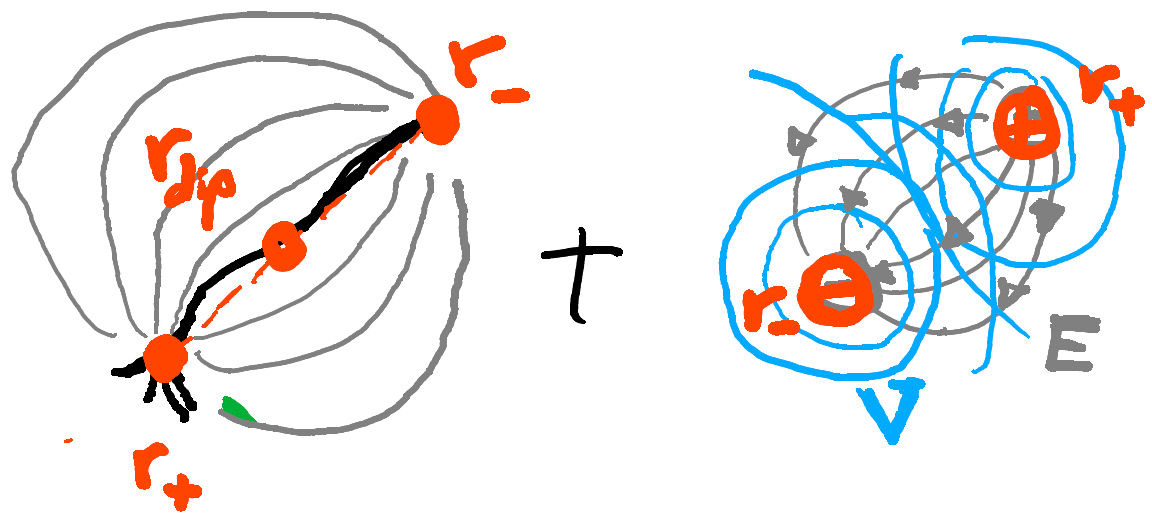
\includegraphics[width=0.4\linewidth]{./img_dev/nsNeuronDipole}
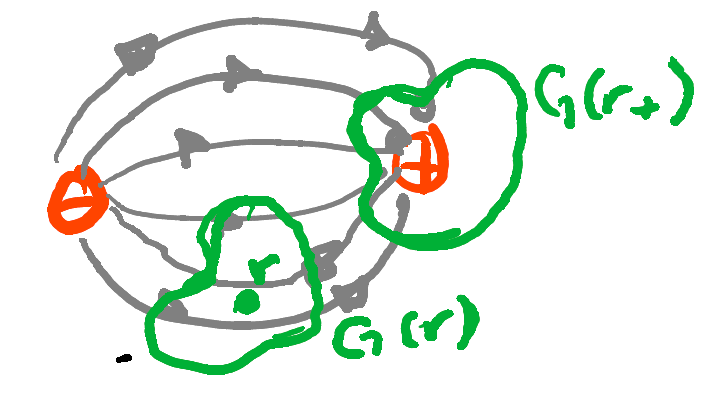
\includegraphics[width=0.4\linewidth]{./img_dev/nsCurrDensField}
\caption{A. The electrical field, $E$, is the gradient of the electric scalar potential field, $V$. In the quasi-static case, we assume that the magnetic field is constant in time, and thus, its influence over the electric fields is negligible. B. The gradient of the electric current density, $K$, banishes everywhere except on the sink and source created by the dipole. }
\label{fig:diagrams1}
\end{figure}

With equations \eqref{eq:model1} and \eqref{eq:model2} at hand, we may determine the electric scalar field, $V$, in terms of the only dipole as
\begin{equation}
\nabla \cdot\ppar{\sigma(\rr)\, \nabla V(\rr) } = 
{\delta\ppar{r-\rr_+} - \delta\ppar{r-\rr_-}}
\label{eq:poisson_gral}
\end{equation}
or, in the isotropic case, as
\begin{equation}
\kappa \Delta V(r) = 
{\delta\ppar{r-\rr_+} - \delta\ppar{r-\rr_-}}
\label{eq:poisson_isotropic}
\end{equation}

It is relevant to recall that the EEG measurement from the only sensor is $V(s)$, with $s$ the sensor's location.

%%%%%%%%%%%%%%%%%%%%%%%%%%%%%%%%%%%%%%%%%%%%%%%%%%%%%%%%
%%%%%%%%%%%%%%%%%%%%%%%%%%%%%%%%%%%%%%%%%%%%%%%%%%%%%%%%

\subsection{Boundary conditions Poisson equation}

To have a meaningful solution for equation \eqref{eq:poisson_gral} or \eqref{eq:poisson_isotropic} in the context of EEG, we must consider appropriate domain and boundary conditions.

Since the electric conductivity of air is very small compared with that of head tissues, it is straightforward to use the subject's head as a domain with reflective boundary conditions. 
%
Thus, the head is divided into a series of nested volumes, determined by both the biological tissues in place and their respective electric properties.

Under these conditions, the simplest model considers a small number of tissue-based regions as homogeneous isotropic media with constant conductivity; different media may have different conductivity.
%
The 4-sphere model considers only four media: the brain, $\mathcal{M}_4$, cerebrospinal fluid (CSF), $\mathcal{M}_3$, skull, $\mathcal{M}_2$, and the rest of the head, $\mathcal{M}_1$.
%
For computational purposes, we may consider a fifth medium, $\mathcal{M}_0$, representing outside of the head.

Multiple approximations are used in practice, as illustrated in figure \ref{fig:diagrams2} where portions of the skull far from the brain are ignored, as well as muscle and connective tissues 
because those tissues are too far from the EEG sensors to make a significant difference in the model.

\begin{figure}
\centering
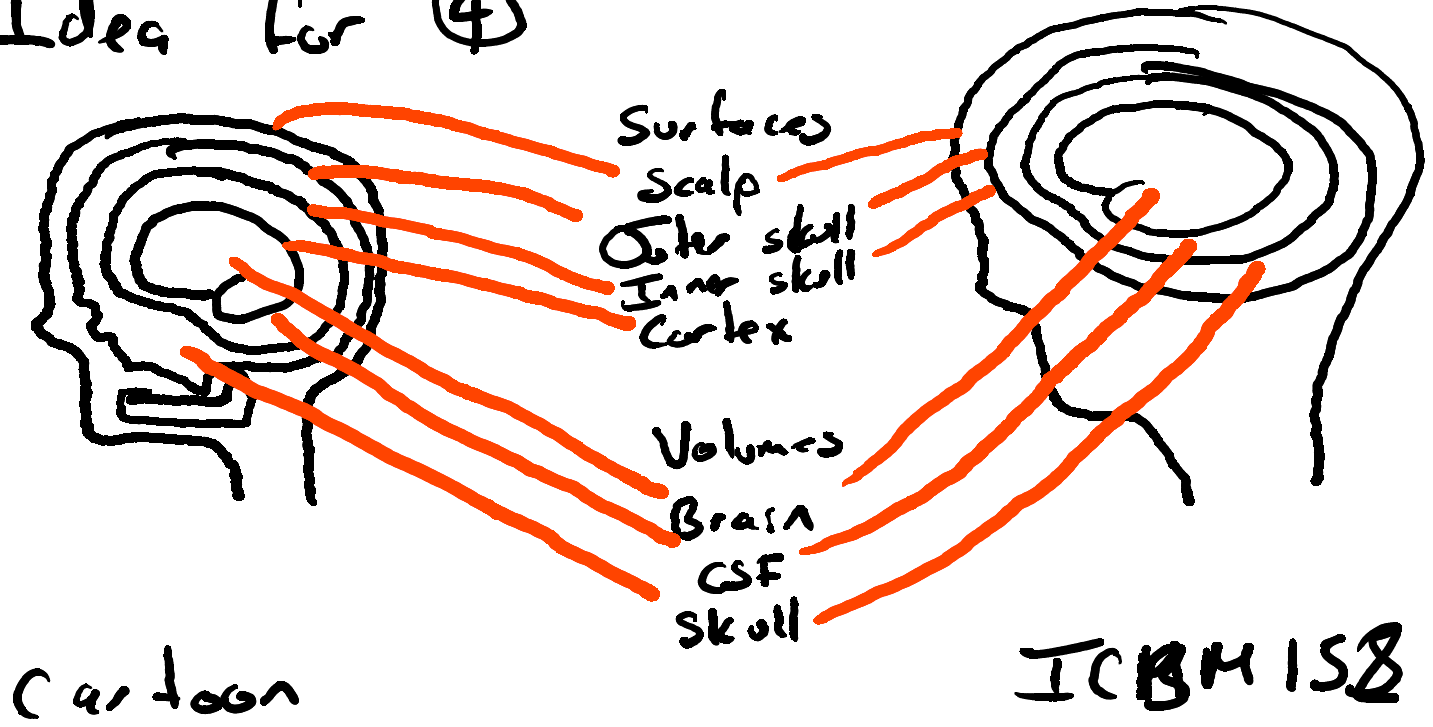
\includegraphics[width=0.8\linewidth]{./img_dev/nsHeadSurfacesVolumes}
\caption{Geometric domain defined by relevant tissues in the subject's head. The 4-sphere model considers three media: brain, cerebrospinal fluid (CSF), and the rest of the head. Relevant interfaces between media are displayed: brain cortex, inner and outer skull, and scalp. (Left) Cartoonish diagram displaying the elements. (Right) Surfaces extracted from the ICBM152 template were included to show realistic proportions.}
\label{fig:diagrams2}
\end{figure}

With the media defined formally, we may state the reflective boundary conditions,
\begin{equation}
\sigma(\rr)\, \nabla V(\rr) \cdot \mathbf{n} = 0, 
\text{ for } \rr \in \mathcal{M}_1
\label{eq:boundary1}
\end{equation}
where $\mathbf{n}$ is a vector orthogonal to $\partial\mathcal{M}_1$.
%
Similarly, boundary conditions at the interfaces are just continuity for the derivative,
\begin{equation}
\left\{
\begin{array}{rl}
\ppar{\lim_{
\rr_i\rightarrow \rr 
\rr_i\in \mathcal{M}_i
}
\sigma(\rr_i)
\, 
\nabla 
V(\rr_i)
} 
\cdot 
\mathbf{n}
&=
\ppar{\lim_{\rr_{i+1}\rightarrow \rr \rr_{i+1}\in \mathcal{M}_{i+1}}
\sigma(\rr_{i+1})\, \nabla V(\rr_{i+1})} \cdot \mathbf{n} 
\\
{\lim_{\rr_i\rightarrow \rr \rr_i\in \mathcal{M}_i}
V(\rr_i)} 
&=
{\lim_{\rr_{i+1}\rightarrow \rr \rr_{i+1}\in \mathcal{M}_{i+1}}
V(\rr_{i+1})} 
\end{array}
\right.
\label{eq:boundary2}
\end{equation}
%\begin{equation}
%tmp
%\label{eq:boundary2}
%\end{equation}
for $\rr \in \mathcal{M}_i \cap \mathcal{M}_{i+1}$, 
with 
$\mathbf{n}$ is a vector orthogonal to
$\rr \in \mathcal{M}_i \cap \mathcal{M}_{i+1}$
and
$i = 1, 2, 3$.

\subsubsection{Practical considerations}

Either equation \eqref{eq:poisson_gral} or \eqref{eq:poisson_isotropic} must be solved within the geometric regions described previously, subject to the boundary conditions \eqref{eq:boundary1} and \eqref{eq:boundary2}.
%
The construction and treatment of those regions and the solution per se require special discussion.

Regions are often defined from the subject's anatomical data or an appropriately matched template.
%
The anatomical information is usually a T1 or T2 MRI, which is later segmented to identify relevant tissues. The segmented MRI is then used to obtain triangulated surfaces. 
%
More media can be incorporated into the model, such as a division of the brain into white matter and grey matter;
Those approaches are limited in the reliability with which these tissues can be identified.

Multiple commercial software is available for the segmentation of MRI and extraction of triangulated surfaces, such as ...

Once the triangulated surfaces are obtained, the equation can be solved numerically by either using Boundary Element Method (BEM), Finite Element Method (FEM), or others.

\subsection{Construction of the leadfield operator}

Recall that both equations \eqref{eq:poisson_gral} and \eqref{eq:poisson_isotropic} are constructed for one sensor and one dipole with unit magnitude.
%
We now consider a large number of EEG sensors at locations $s_1, s_2, \dots, s_M \in \R^3$, and dipoles at locations $d_1, d_2, \dots, d_N \in \R^3$
with magnitudes $m_1, m_2, \dots, m_N$.
%
By making the same assumptions and formulations as in the previous sections, the conclusion is that the electric scalar field under these new circumstances is given by
\begin{equation}
V(r) = 
\sum_{n=1}^N m_n \tilde{V}_{d_n}(r)
\end{equation}
where $\tilde{V}_n$ is the solution to 
\begin{equation}
\nabla \cdot\ppar{\sigma(\rr)\, \nabla \tilde{V}(\rr) } = 
{\delta\ppar{r-d_n^+} - \delta\ppar{r-d_n^-}}
\end{equation}
under the boundary conditions \eqref{eq:boundary1} and \eqref{eq:boundary2}, and with $d_n^\pm$ constructed from $d_n$.

For ease of notation, define 
\begin{align}
g(r, d) &= \tilde{V}_d(r)
\end{align}
and thus, we can write
\begin{equation}
V(r) = 
\sum_{n=1}^N m_n g\ppar{r, d_n} = 
\spar{g\ppar{r, d_1}, g\ppar{r, d_2}, \cdots, g\ppar{r, d_N}}
\spar{m_1, m_2, \cdots, m_N}\trans
\label{eq:back1}
\end{equation}
Furthermore, by using the equation for all the sensor locations and stacking the results, we obtain the following vector equation
\begin{equation}
\begin{bmatrix}
V\ppar{s_1} \\
V\ppar{s_2} \\
\vdots
V\ppar{s_M}
\end{bmatrix}
=
\begin{bmatrix}
\spar{g\ppar{s_1, d_1}, g\ppar{s_1, d_2}, \cdots, g\ppar{s_1, d_N}} \\
\spar{g\ppar{s_2, d_1}, g\ppar{s_2, d_2}, \cdots, g\ppar{s_2, d_N}} \\
\vdots \\
\spar{g\ppar{s_M, d_1}, g\ppar{s_M, d_2}, \cdots, g\ppar{s_M, d_N}}
\end{bmatrix}
\label{eq:model3}
\end{equation}

Equation \eqref{eq:model3} can be rewritten as the following generic matrix equation
\begin{equation}
\Y = \G\, \J
\label{eq:model4}
\end{equation}
where $\Y \in \R^{M\times 1}$ is a vector of EEG measurements, $\J \in \R^{N\times 1}$ is a vector of dipole magnitudes, and $\G \in \R^{M\times N}$ is a matrix known as the leadfield matrix, gain matrix, forward operator, among other names.

The forward model can be extended trivially to account for $T$ EEG measurements in time by setting $\Y \in ]R^{M\times T}$, $\Y \in \R^{M\times T}$, and $\G$ unchanged.


If the dipole's orientation is to be determined, then we can consider each dipole as the sum of three dipoles parallel to some orthogonal directions. Such as in figure \ref{fig:diagrams3}, we can write
\begin{equation}
m_n d_n = m_n^x e_n^x + m_n^y e_n^y + m_n^z e_n^z
\end{equation}
with $e_n^x, e_n^y, e_n^z \in \R^3$ unit-norm vectors located at $d_n$ and parallel to the respective $x-, y-, z-$axis.
%
Under these new circumstances, equation \eqref{eq:back1} changes to
\begin{equation}
V(r) = 
\sum_{n=1}^N \ppar{m_n^x g\ppar{r, e_n^x} + m_n^y g\ppar{r, e_n^y} + m_n^y g\ppar{r, e_n^y}
}
\end{equation}
which can be written as a matrix equation such as \eqref{eq:model4}.

The overall effect of assuming unknown orientations are (1) the increase of the number of dipole magnitudes to be determined by a factor of 3, as well as the size of the leadfield matrix, and (2)
we need to compute the magnitude of these dipoles in order to recover the original interpretation.

\begin{figure}
\centering
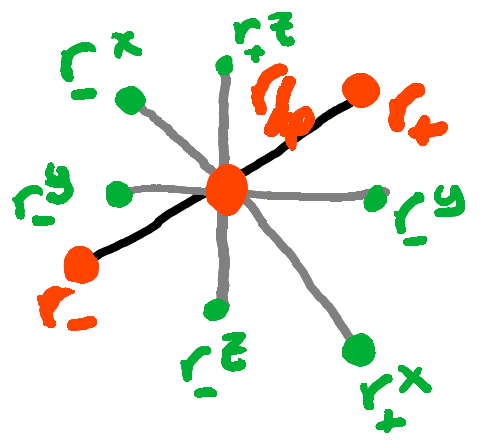
\includegraphics[width=0.4\linewidth]{./img_dev/nsOrthDecomp}
\caption{Decomposition of an arbitrary dipole as a sum of projections into the three canonical directions.}
\label{fig:diagrams3}
\end{figure}

\section{Limitations of surface electrodes}



There are several neural activity patterns that surface electrodes cannot represent properly.
%
Silent activity refers to neural activity that doesn't produce a significant electric potential and is not registered by surface electrodes.
%
It is estimated that only 20\% of the brain's energy is spent producing non-silent activity.

The orientation of neuron dendrites, which carry the post-synaptic potentials, plays a key role in how much of their activity is recorded by surface electrodes.
%
Pyramidal neurons at the gray matter (located at the outer cortex) are almost exclusively oriented parallel to the cortex surface.
%
This common orientation, combined with their physical proximity to the scalp, makes the pyramidal neurons to be over-represented on recordings from surface electrodes.

On the other side, neural activity occurring at the lower layers of the brain is more difficult to register and reconstruct.

These limitations of this recording modality are inherited from the ESI methods, and thus, they must be considered when interpreting the obtained results.

A second set of limitations from the model of distributed dipoles, which represent a spatial average of the .
%
Distributed dipoles can efficiently represent synchronous activity over large regions, a phenomenon known as a source patch.
%
Distributed dipoles of low magnitude may represent smaller source patches and regions with asynchronous orientations, resulting in .




%An important consideration in the practice is the location of the dipoles. 
%
The distributed dipole model is agnostic in that it doesn't make any assumptions about the location of the dipoles.
%
A region with no active dipoles leads to equivalent dipoles with zero magnitude, while a region with active dipoles leads to equivalent dipoles with non-zero magnitude.